%%%%%%%%%%%%%%%%%%%%%%%%%%%%%%
% 	   美赛模板,正文部分		 
%          PAPER.tex         
%%%%%%%%%%%%%%%%%%%%%%%%%%%%%%

\documentclass[12pt]{article}

% 请在此填写控制号、题号和标题,年份不需要填(自动以当前电脑时间年份为准)
\usepackage{graphicx}
\usepackage[1591]{easymcm}\problem{A}   
\usepackage{palatino} % 这个是COMAP官方杂志采用的字体,如不需要可注释掉,以使用默认字体
\usepackage{booktabs}  %  引入三线表宏包
\usepackage{pgfplots}
\usepackage{longtable} % 跨页宏包
\usepackage{pgfplotstable}
\title{An MCM Paper Made by Team 1591}  % 标题

% 如您参加的是ICM(即选择了D/E/F题),请使用以下的命令修改Summary Sheet题头
% \renewcommand{\contest}{Interdisciplinary Contest in Modeling (ICM) Summary Sheet}

% 正文开始
\begin{document}
	%%%%%%%%%%%%%%%%%%%%%%%%%%%%%%%%%%%%%%%%%
%%            请在此填写摘要            %%
%% 请勿编译/排版此文件,请编译PAPER.tex!  %%
%%%%%%%%%%%%%%%%%%%%%%%%%%%%%%%%%%%%%%%%%
\begin{abstract}\small
	
	In the carbon cycle process, the decomposition of organic matter, especially the degradation of plant material and woody fibers involving fungi, is an essential link. We explore the relationship between fungal properties (growth rate and moisture resistance) and the decomposition rate of wood fibers to better understand the relationship and mechanism between the degradation of plant material and woody fibers and fungi. \par 
	Firstly, considering multiple factors, through data-based regression analysis, we initially establish a multiple linear regression model of the decomposition rate of wood fiber, and explain the rationality of the model from the perspective of biology and ecology. At the same time, from a mathematical point of view, we established a mathematical model containing an exponential relationship between fungal growth rate and fungal moisture resistance-the fungal growth rate model, which correlates these two biological characteristics of fungi. And the actual data verifies the rationality of this model. \par 
	Secondly, the decomposition of wood fibers by fungi in nature is often the result of the joint action of different populations and there are also interactions between fungal populations, Therefore, we use the growth rate and moisture resistance of fungi as the standard according to the K-Means clustering algorithm and the elbow rule to cluster fungi. In order to analyze the interactions within and between the fungal categories. Then, we optimized and improved the previously established fungal growth rate model based on the Monod equation in microbial dynamics and the theory of interaction between populations, and obtained a fungal growth rate model combined with interaction. We verify the rationality of the model by listing examples of interacting fungal populations under ideal conditions. The final result achieves the unity of theory and practice.\par 
	Thirdly, according to the optimized fungal growth model. We discuss and analyze the dynamics of the interactions in terms of long-term and short-term action time, revealing the principles of these two phenomena in nature. In addition, we analyzed the sensitivity of the model to rapidly changing natural conditions and tried to explain it from a biological perspective.\par 
	Then,in predicting the strengths and weaknesses of each fungal group and the likely combinations of fungi to survive, we considered the possible conditions in different climatic environment,including arid, semiarid, temperate, arboreal, and tropical rain forests.Combined with the analysis and experimental data of previous papers, we concluded that fungi with a high growth rate and moisture tolerance are more likely to survive when the environment is relatively stable.While when the weather is changeable,fungi with a large water niche width are more competent.We also further discussed the dependence between fungi and the environment and found out the possible seasonal changes of fungi in different areas.\par 
	Finally,our model successfully shows the relationship between fungal species diversity and decomposition rate. When the fungal species diversity is higher, the decomposition rate will also decrease. Because decomposition will emit carbon dioxide, it also indirectly implies the relationship between species diversity and carbon dioxide. It has positive significance for environmental issues related to greenhouse gas emission reduction, and is helpful to optimize the global carbon cycle and co-build a beautiful earth.\par 


    % 美赛论文中无需注明关键字。若您一定要使用,
    % 请将以下两行的注释号'%'去除,以使其生效;
    % 若您不使用,可直接将这段注释删除
    % \vspace{5pt}
    % \textbf{Keywords}: MATLAB, mathematics, LaTeX.

\end{abstract}




%%%%%%%%%%%%%%%%%%%%%%%%%%%%%%%%%%%%%%%%%%
% 如不理解以下部分中各命令的含义,请勿修改! %
%%%%%%%%%%%%%%%%%%%%%%%%%%%%%%%%%%%%%%%%%%

%---------以下生成sheet页----------
% 下面的语句可调整全文行距为标准值的0.6倍,请自行使用
% \renewcommand{\baselinestretch}{0.6}\normalsize
\maketitle  			% 生成sheet页
\thispagestyle{empty}   % 不要页眉页脚和页码
\setcounter{page}{-100} % 此命令仅是为了避免页码重复报错,不要在意

%---------以下生成目录----------
\newpage
\tableofcontents
\thispagestyle{empty}   % 不要页眉页脚和页码
\newpage

%---------以下生成正文----------
\setlength\parskip{0.8\baselineskip}  % 调整段间距
\setcounter{page}{1}    % 从正文开始计页码
\pagestyle{fancy}		% 摘要请到ABSTRACT.tex中填写
	
	\section{Introduction}
	\subsection{Problem Background}
	Here is the problem background ...
	
	Two major problems are discussed in this paper, which are:
	\begin{itemize}
		\item Doing the first thing.
		\item Doing the second thing.
	\end{itemize}
	
	\subsection{Literature Review}
	A literatrue\cite{1} say something about this problem ...
	
	\subsection{Our work}
	We do such things ...
	
	\begin{enumerate}[\bfseries 1.]
		\item We do ...
		\item We do ...
		\item We do ...
	\end{enumerate}
	
	\section{Preparation of the Models}
	\subsection{Assumptions}
	
	\subsection{Notations}
	The primary notations used in this paper are listed in \textbf{Table \ref{tb:notation}}.
	
	%\begin{center}
	%	\begin{spacing}{1.1}
	%		%longtable的意思是 这个表格可以跨页
	%		\begin{longtable}{p{.1\textwidth}p{.7\textwidth}m{.3\textwidth}}
	%			\caption{description}
	%			\label{table1}
	%			\toprule   %第一行线
	%			%表示第一列占1.5cm 第二列占6cm 第三列占2cm 的距离 并且这几个字都是居中对齐
	%			\multicolumn{1}{m{1.5cm}}{\centering Symbol} & \multicolumn{1}{m{6cm}}{\centering Definition} & \multicolumn{1}{m{2cm}}{ Unit} \\
	%			\midrule   %第二行线
	%			$V$ & index & -- \\
	%			$X$ & The  & -- \\
	%			$Y$ & The & -- \\
	%			$Z$ & The  & -- \\
	%			\bottomrule   %第三行线
	%		\end{longtable}
	%	\end{spacing}
	%\end{center}
	
	\begin{center}
		\setlength{\tabcolsep}{0.7mm}{
			\begin{longtable}{ll}
				\caption{Notations}
				\label{tb:notation}\\
				\toprule  % 顶部线
				Definition&Symbol\\ 
				\midrule  % 中部线
				Decomposition rate&$D$ \\
				The decomposition donated by the \emph{i} th specices of fungi&$D_i$\\
				Regression coefficient&$\alpha_{ij}$\\
				The growth rate of the \emph{i} th specices of fungi&$E_i$ \\
				Moisture tolerance&$M$ \\
				Moisture tolerance of the \emph{i} th specices of fungi &$M_i$ \\
				Temperature seasonality&$T_s$ \\
				Temperature annual range&$T_R$ \\
				Percipitation of westtest quarter&$P_w$\\
				\bottomrule  % 底部线
			\end{longtable}
		}
	\end{center}
	
	%\begin{longtable}[htbp]
	%	\centering
	%	\caption{Notations}
	%	\begin{tabular}{ll}
	%		\toprule  % 顶部线
	%		Definition&Symbol\\ 
	%		\midrule  % 中部线
	%		Decomposition rate&$D$ \\
	%		The decomposition donated by the \emph{i} th specices of fungi&$D_i$\\
	%		Regression coefficient&$\alpha_{ij}$\\
	%		The growth rate of the \emph{i} th specices of fungi&$E_i$ \\
	%		Moisture tolerance&$M$ \\
	%		Moisture tolerance of the \emph{i} th specices of fungi &$M_i$ \\
	%		Temperature seasonality&$T_s$ \\
	%		Temperature annual range&$T_R$ \\
	%		Percipitation of westtest quarter&$P_w$\\
	%		\bottomrule  % 底部线
	%	\end{tabular}\label{tb:notation}
	%\end{longtable}
	
	%\begin{table}[!htbp]
	%\begin{center}
	%\caption{Notations}
	%\begin{tabular}{cl}
	%	\toprule
	%	\multicolumn{1}{m{3cm}}{\centering Symbol}
	%	&\multicolumn{1}{m{8cm}}{\centering Definition}\\
	%	\midrule
	%	$D$&Decomposition rate\\
	%	$D_i$&The decomposition donated by the \emph{i} th specices of fungi\\
	%
	%    $\alpha_{ij}$&Regression coefficient\\
	%	\bottomrule
	%\end{tabular}\label{tb:notation}
	%\end{center}
	%\end{table}\par
	
	\section{The Preliminary Model}
	\subsection{Carbon cycle and fungi}
	The carbon cycle describes the cycle of exchange of carbon in the biosphere, lithosphere, hydrosphere, and atmosphere.As one of the most important cycles on Earth, the process of the carbon cycle can be described as the absorption of carbon dioxide from the atmosphere by plants on land and in the sea, through biological or geological processes and human activities, and then returned to the atmosphere as carbon dioxide.(See Figure 1 for details.)\par
	
	
	In the process of biological participation in the carbon cycle, one of the main activities is microbial participation in the decomposition of compounds, which changes the form of carbon element to participate in the carbon cycle.A key component in this process is the decomposition of plant material and wood fibers, with fungi being the main factor in the decomposition of wood fibers.\\
	
	% h默认参数是可以浮动,不是固定在当前位置。如果要不浮动,你就可以使用大写float宏包的H参数,固定图片在当前位置,禁止浮动。
	% [ht]是可选项 h表示的是here在这里插入,t表示的是在页面的顶部插入
	% h 此处(here)t 页顶(top)b 页底(bottom)p 独立一页(page)
	
	\begin{figure}[h] % h为当前位置,!htb为忽略美学标准,htbp为浮动图形
		\centering
		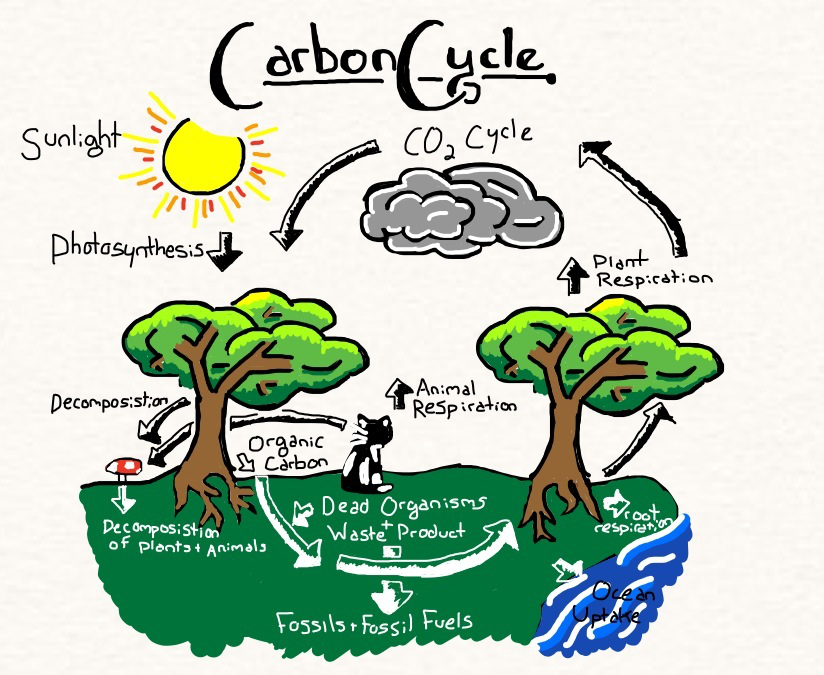
\includegraphics[width=8cm]{carboncycle.jpg}
		\caption{carbon cycle}
	\end{figure}
	
	
	
	\subsection{Construction of fungal growth rate model}
	\subsubsection{Brief introduction of modeling process}
	In order to understand how fungi are involved in the decomposition of plant materials and wood fibers, it is necessary to understand the biological characteristics of the fungi involved in the decomposition -- the growth rate of the fungi.Consequently, we should model the growth rate of the fungus first.This step is not unnecessary and will be crucial to our understanding and subsequent modeling.\par
	We took the following steps to model the growth rate of the fungus.
	
	
	\begin{enumerate}[\bfseries 1.]
		\item Step 1: According to the data provided by the data set, the multiple linear regression model between the growth rate and factors that may be related was constructed. Besides, preliminary screening was conducted to obtain the main variables that affect the growth rate according to the significance level of each independent variable.
		\item Step 2: The main variables screened out in Step 1 will be verified and interpreted from the biological perspective according to relevant literature. Variables lacking rationality will be excluded. Finally, we will establish the multiple linear regression model of fungi.
	\end{enumerate}\par
	
	\subsubsection{Verify and interpret mechanism}
	
	We carefully analyzed the data of the relationship between moisture tolerance and decomposition rate given in the question, and found that moisture tolerance had a significant impact on decomposition rate. In order to prove our point of view, we draw the \textbf{figure \ref{figure:moisture_tolerance_growth_rate}} of moisture tolerance and growth rate, because growth rate will affect decomposition rate. If we find a significant relationship between moisture tolerance and growth rate, we can infer that there is a relationship between moisture tolerance and decomposition rate. This hypothesis is also consistent with the findings of Daniel S. Maynard et al.\cite{3}, whose analysis revealed a fundamental balance between moisture tolerance and competitiveness, i.e., fungi with broad thermal and water niches exhibit low displacement capacity. The magnitude of this tolerance tradeoff is partly related to the environmental conditions in which the fungi are located, in which the thermal niche traits show the strongest climatic relationship.
	\begin{figure}[h]
		\centering
		\begin{tikzpicture}
			\begin{axis}[xlabel = moisture tolerance, ylabel = growth rate]
				\addplot [domain=-1:1, only marks, mark size=0.9pt] table {moisture_tolerance_growth_rate.txt};
				\addplot [domain=-1:1, red] {1.0506*exp(2.3945*x)};
			\end{axis}
		\end{tikzpicture}
		\caption{growth rate curve of moisture tolerance}
		\label{figure:moisture_tolerance_growth_rate}
	\end{figure}
	
	
	%After the significance analysis of multiple regression, it was found that the mycelium density, the optimal temperature, the optimal humidity growth rate, and the precipitation of the wettest month had a significant effect on the growth rate of the fungus.We tried to analyze theoretically why these four variables would have a significant effect on the growth rate of the fungus.\par
	%
	%1.Mycelium density——The significant effect of mycelium density on the growth rate is not beyond our expectation, and is consistent with our conclusions from previous studies of researchers, and is consistent with Lynne Boddy's hypothesis in the paper that dense mycelium will reduce the decomposition rate of wood.We've also come up with a couple of possible hypotheses.One is the nutrient competition among hyphae——hyphae grow at a fast rate which results in the rapid decrease of some necessary reactive substances in the soil because they are not replenished. It may also be that the production rate of such substances exceeds the consumption rate. Another hypothesis is that the decomposition reaction is exothermic. Due to the high density of mycelia and the fast growth rate, the decomposition reaction is intensified and the exothermic increase which results in the loss of enzyme activity in the soil, and the fragile mycelia die because they cannot absorb enough nutrients.\par
	%
	%2.The best temperature——Temperature can significantly increase the activities of enzymes in the soil, so that the activities of enzymes reach the maximum at the appropriate temperature.The optimum temperature reflects the adaptation of fungi to the ambient temperature, and when the optimum temperature is in the temperature range where enzymes remain active, it can just accelerate the rate of nutrient absorption by fungi.If the temperature is high enough, the plant can take advantage of the high activity of enzymes in the soil at higher temperatures, gain better survival ability in the harsh natural environment, can maintain competitiveness over a larger range, and accelerate the growth rate of fungi.Using data from Daniel S. Maynard et al., we also plot the relationship between optimal temperature and competitive ranking, and using linear fitting, we find that the higher the optimal temperature, the faster the growth rate, and the higher the ranking of fungi, which is consistent with our initial hypothesis.\par
	%
	%3.Optimal humidity growth rate——The higher the growth rate, the higher the natural optimum humidity growth rate.The two concepts are very similar.By linear fitting, it is found that there is almost a direct ratio relationship.\par
	%
	%4.Precipitation in the wettest months--The wettest months are the time of year when the rainfall is the highest, which represents the amount of annual rainfall to some extent. If the wettest months do not meet the humidity and water needed for fungal growth, the growth rate of the fungus will be reduced.Therefore, if the rainfall is higher, the air is more likely to reach the humidity required by the fungus, and it is more likely to maintain the humidity required by the fungus for a longer period of time, thus accelerating the growth rate of the fungus. Our hypothesis results are consistent with the simulation results of our model.
	
	\subsubsection{Simplified to mathematical model}
	Set E as the growth rate, a, b, c as constants, and m as moisture tolerance.
	\begin{equation}
		\begin{array}{l}
			E=ae^{bM} + C
		\end{array}
	\end{equation}
	
	\subsection{Construction of decomposition rate model}
	\subsubsection{Brief introduction of modeling process}
	In order to understand how fungi are involved in the decomposition of plant materials and wood fibers, it is necessary to understand the biological characteristics of the fungi involved in the decomposition -- the growth rate of the fungi.Consequently, we should model the growth rate of the fungus first.This step is not unnecessary and will be crucial to our understanding and subsequent modeling.\par
	We took the following steps to model the growth rate of the fungus.
	\begin{enumerate}[\bfseries 1.]
		\item According to the data provided by the data set, the multiple linear regression model between the growth rate and factors that may be related was constructed. Besides, preliminary screening was conducted to obtain the main variables that affect the growth rate according to the significance level of each independent variable.
		\item The main variables screened out in Step 1 will be verified and interpreted from the biological perspective according to relevant literature. Variables lacking rationality will be excluded. Finally, we will establish the multiple linear regression model of fungi.
	\end{enumerate}
	\subsubsection{Verify and interpret mechanism}
	Having established and completed the mathematical model of the growth rate, we then proceeded to establish the mathematical model of the decomposition rate.Four variables—growth rate, temperature seasonality, annual temperature range, and rainfall in the wettest months, were found to have significant effects on fungal decomposition rate, i.e., 122 day residual mass, by multiple regression analysis of significance.We have tried to analyze from a theoretical point of view why these four variables have a significant effect on the decomposition rate.
	\par
	
	1.Growth rate——Fungi need to absorb nutrients from substrates for growth, and the speed of growth reflects the speed of absorption of nutrients by fungi.McGuire and Kristal pointed out in their paper that in classical competition theory\cite{4}, when organisms have similar ecological characteristics, competition for a resource either maintains diversity through niche differentiation or leads to the loss of diversity through the extinction of inferior competitors. Exploitation competition, in which one microbe takes up a resource faster than another, allows a fungus to absorb nutrients more quickly as its growth rate increases.The growth rate was a significant factor in the decomposition rate.\par
	
	2.Temperature seasonality——The seasonality of temperature reflects the temperature difference throughout the year, but if the temperature difference is too large, the growth rate of fungi will be affected. Through the linear model, we can preliminarily understand that when the temperature difference is too large throughout the year, the growth rate will decrease, and we can also conclude that when the growth rate of fungi slows down, the decomposition rate of fungi will be significantly reduced.So temperature seasonality will also be a significant factor in our model.\par
	
	\begin{figure}[ht]
		\centering
		\begin{tikzpicture}
			\begin{axis}[xlabel = Temperature seasonality, ylabel = growth rate]
				\addplot [domain=0:11000, only marks, mark size=0.9pt] table {Temperature_Seasonality_growth_rate.txt};
				\addplot [domain=0:11000, red] {126.06*exp(-0.483*ln(x))};
			\end{axis}
		\end{tikzpicture}
		\caption{growth rate curve of Temperature seasonality}
		\label{figure:Temperature_Seasonality_growth_rate}
	\end{figure}
	
	\subsubsection{Simplified to mathematical model}
	\begin{equation}
		\begin{cases}
			D=\sum\limits_{i=1}^{n}D_i\\
			D_i=\alpha_{i1} E_i+\alpha_{i2} T_s+\alpha_{i3}T_R+\alpha_{i4}P_w\\
			%E_i=E_i(M_i,T,P)\\
		\end{cases}
	\end{equation}
	
	
	
	
	\section{The Interactions Between Different Species of Fungi}
	Part I: Fungi classification.\par
	In order to further understand the interaction between fungal populations, K-means clustering, systematic clustering algorithm and elbow rule were adopted to conduct cluster analysis according to the characteristics of fungi themselves.
	The detailed flow chart is as follows.\par
	
	
	The pedigree diagram obtained by the system clustering algorithm.\par
	
In order to obtain the optimal number of clustering K,we compared the aggregation coefficients of different cluster numbers, and obtained the final optimal number of clusters by elbow rule is 4 (K=4).The classification of these four types of fungi.
	Based on the above clustering results, we can make the following assumptions.\par
	
	1. Fungi belonging to the same category, which have highly similar biological traits, play similar roles in the decomposition process of wood fibers.
	2. Different types of fungi, including those with relatively low similar biological traits, play different roles in the decomposition of wood fibers.
	
	
	The merging of fungal interactions
	In the previous part, we gave a specific classification of fungi......
	Now let's look at the interaction between fungi in two ways.
	For fungi of the same class, due to the high similarity of biological characters, the same class also showed similar relationship in the decomposition process of wood fiber.
	Therefore, in order to simplify the model and further analysis, we adopted the following operation: the fungi closest to the cluster center in each category were selected as the representative of this category.Since the influence of similarity plays a major role, the differences within categories can be ignored.
	
	
	For fungi between different classes
	Fungi of different categories have low similarity in their biological traits. On the one hand, they undertake different tasks in the decomposition process of wood fibers; on the other hand, they compete for resources, which is directly reflected in the influence of their respective growth rates.
	In fact, based on the data set provided and the literature, we can modify the mycelium density term in the fungal growth rate model and take into account the evolution of the population.
	
	
	Part three: the optimization of the preliminary model
	In the previous chapter, we have obtained the models of fungal growth rate and lignofiber decomposition rate. Obviously, this model does not take into account the interaction between fungi, which is still discrepant from the real model.
	In this chapter, we carry out specific analysis, take into account the interaction within and between populations, and extend the preliminarily established multiple linear regression model to the generalized multiple linear regression model.
	
	
	The final optimization model can be obtained as follows
	
	
	
	
	
	
	
	
	
	
	
	
	
	
	
	
	
	
	
	
	
	
	
	
	
	
	
	
	
	
	
	
	
	
	
	
	
	
	
	
	
	
	
	
	
	\section{Strengths and Weaknesses}
	\subsection{Strengths}
	\begin{itemize}
		\item First one...
		\item Second one ...
	\end{itemize}
	
	\subsection{Weaknesses}
	\begin{itemize}
		\item Only one ...
	\end{itemize}
	
	\begin{thebibliography}{99} 
		\addcontentsline{toc}{section}{References}  %引用部分标题("Refenrence")的重命名
		\bibitem{1}Elisa T. Lee, Oscar T. Survival Analysis in Public Health Research. \emph{Go. College of Public Health}, 1997(18):105-134.
		\bibitem{2}Wikipedia: Proportional hazards model. 2017.11.26. \texttt{\\https://en.wikipedia.org/wiki/Proportional\_{}hazards\_{}model}
		\bibitem{3}D. S. Maynard et al., Consistent trade-offs in fungal trait expression across broad
		spatial scales. Nat. Microbiol. 4, 846–853 (2019).
		\bibitem{4}K. L. McGuire, K. K. Treseder, Microbial communities and their relevance for ecosystem models: Decomposition as a case study. Soil Biol. Biochem. 42, 529–535 (2010).
		\bibitem{5}
		\bibitem{6}
		\bibitem{7}
		\bibitem{8}
		\bibitem{9}
		\bibitem{10}
		\bibitem{11}
		\bibitem{12}
		\bibitem{13}
		\bibitem{14}
	\end{thebibliography}
	
	
	% ==============以下为附录内容,如您的论文中不需要程序附录请自行删除====================
	\clearpage
	\begin{subappendices}						% 附录环境
		\section*{Apendix: The source codes}		% 附录标题可以自行修改
		\addcontentsline{toc}{section}{Appendix}  	% 将附录内容加入到目录中
		
		This MATLAB program is used to calculate the value of variable $a$.
		\begin{lstlisting}[language=Matlab, caption=\texttt{temp.m}]
			a = 0;
			for i = 1:5
			a = a + 1;
			end
		\end{lstlisting}
		
		This LINGO program is used to search the optimize solution of 0-1 problem.
		\begin{lstlisting}[language=Lingo, caption=\texttt{temp.lg4}]
			model:
			sets:
			WP/1..12/: M, W, X;
			endsets
			data:
			M = 2 5 18 3 2 5 10 4 11 7 14 6;
			W = 5 10 13 4 3 11 13 10 8 16 7 4;
			enddata
			max = @sum(WP:W*X);
			@sum(WP: M * X)<=46;
			@for(WP: @bin(X));
			end
		\end{lstlisting}
		
	\end{subappendices}
	% =================================================================================
	
	
	
\end{document}